\documentclass{beamer}


%\beamertemplateshadingbackground{yellow!100}{white}
\usepackage[english]{babel}
\usepackage{amsfonts,amsmath}
\usepackage{graphicx}
\graphicspath{{figures/}} % Location of the graphics files
\usepackage{sansmathaccent}
\pdfmapfile{+sansmathaccent.map}


%\usetheme{Warsaw}
\usetheme[secheader]{Madrid}

\usepackage{multimedia}
\logo{
\includegraphics[height=0.5cm]{imi.jpg}}

\newcommand{\be}{\begin{equation}}
\newcommand{\ee}{\end{equation}}
\newcommand{\rf}[1]{(\ref{#1})}
\newcommand{\RR}{\mathbb{R}}
\newtheorem{thm}{Theorem}
\newtheorem{lm}{Lemma}

%\def\ra#1\{\renewcommand{\arraystretch}{#1}
\begin{document}
 %[propagating wave solutions to the 2D BPE]



%---------- frame 01 ----------------
\begin{frame}
\title{Energy Saving Method with Conservative Scheme for the Solution of 2D Boussinesq Paradigm Equation}

\author[K. Angelow]{{\underline{Krassimir Angelow}}, Natalia Kolkovska}
\institute[IMI -- BAS]{Institute of Mathematics and Informatics\\ Bulgarian Academy of Sciences, Sofia, Bulgaria,\\ e-mail: angelow@math.bas.bg}
%\date[2021]{AMITANS, June 20-25  2021,  Albena, Bulgaria}
 \titlepage

\end{frame}

%---------- frame 02 ----------------
\begin{frame}
\tableofcontents 
\setbeamertemplate{table of contents shaded}[default]
\section{Boussinesq Paradigm Equation}
\section{Integral and Energy Formulae}
\section{Energy Saving Method with Conservative Scheme}

\section{Results}

\end{frame}

%---------- frame 03 ----------------
\begin{frame}
\frametitle{Boussinesq Paradigm Equation}


We study the problem

\be\label{problem}
\beta(E-\Delta) \frac{\partial^2 u}{\partial t^2}=
 \beta \Delta u -\Delta^2 u -\alpha \beta \Delta (u^2)
\ee
where $\alpha>0$, $\beta>0$  are dispersion parameters, and $\Delta$ is the Laplace operator.
\end{frame}



%---------- frame 04 ----------------
\begin{frame}
\frametitle{Integral and Energy Formulae}
The integral:

\begin{equation}\label{int}
D(u)=\int_{R^2} u(x,y)dx dy
\end{equation}

and energy:
\begin{align}\label{ex-en}
E(u)=&\int_{R^2} u_t \left((A^{-1}+E)u_t\right) dxdy+
\beta \int_{R^2} u^2 dxdy \nonumber\\
+& \int_{R^2}u \left(A u\right) dxdy
-\frac{2 \alpha \beta}{3} \int_{R^2} u^3 dxdy =const
\end{align}
of the continuous problem \rf{problem}. Here $E(u)$ is the exact energy of problem \rf{problem} and $Au=-\Delta u$.
\end{frame}

\begin{frame}
\frametitle{Energy Saving Method with Conservative Scheme}
\framesubtitle{The Grid}

\begin{center}\vspace{0.4cm}
	\begin{minipage}[b]{0.6\linewidth}
		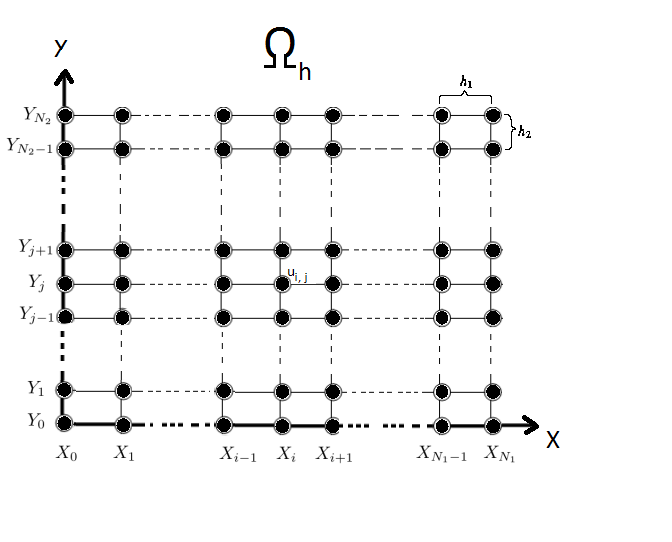
\includegraphics[width=\linewidth]{Omega_dah.png}
	\end{minipage}
\end{center}

\end{frame}


\begin{frame}
\frametitle{Energy Saving Method with Conservative Scheme}


The approximation of the differential operators is defined as:
\begin{equation}
\frac{\partial^2 u}{\partial t^2}(x_i, y_j, t_k ) = \frac{ u^{(k+1)}_{i, j} - 2u^{(k)}_{i,j} + u^{(k-1)}_{i,j} }{\tau^2} + O(\tau^2) 
\end{equation}

\begin{equation}
\frac{\partial^2 u}{\partial x^2}(x_i, y_j, t_k ) = \frac{ u^{(k)}_{i+1, j} - 2u^{(k)}_{i,j} + u^{(k)}_{i-1,j} }{h_1^2} + O(h_1^2) 
\end{equation}

\begin{equation}
\frac{\partial^2 u}{\partial y^2}(x_i, y_j, t_k ) = \frac{ u^{(k)}_{i, j+1} - 2u^{(k)}_{i,j} + u^{(k)}_{i,j-1} }{h_2^2} + O(h_2^2) 
\end{equation}


\begin{equation}
\Delta_h = \frac{ u^{(k)}_{i+1, j} - 2u^{(k)}_{i,j} + u^{(k)}_{i-1,j} }{h_1^2} + \frac{ u^{(k)}_{i, j+1} - 2u^{(k)}_{i,j} + u^{(k)}_{i,j-1} }{h_2^2}
\end{equation}

\end{frame}

\begin{frame}
\frametitle{Energy Saving Method with Conservative Scheme}
The grid function is defined as:
\begin{equation}
(I-\Delta_h)\frac{ u^{(k+1)}_{i, j} - 2u^{(k)}_{i,j} + u^{(k-1)}_{i,j} }{\tau^2} = (\Delta_h - \Delta_h^2)u^{(k)}_{i,j} + \Delta_h(g(u^{(k)}_{i,j}))
\end{equation}
%
where the non-linear term $g$ is defined as:
\begin{align}
g(u^{(k)}_{i,j})=&\frac{\alpha \beta} { 3 } \left( (u^{(k+1)}_{i,j})^2 + (u^{(k-1)}_{i,j})(u^{(k+1)}_{i,j}) + (u^{(k-1)}_{i,j})^2 \right) + \nonumber\\
+&\frac{ (\beta - 1 )}{ 2 }\left( u^{(k+1)}_{i,j} + u^{(k-1)}_{i,j} \right).
\end{align}


\end{frame}

\begin{frame}
\frametitle{Energy Saving Method with Conservative Scheme}
The last transforms into an implicit equation system $M v^{(k+1)} = b( v^{(k+1)} ,  v^{(k)} ,  v^{(k-1)}  )$.

Piccardi  Iterations:

Set
\begin{align}
 v^{(k+1)}_0 =  v^{(k)}
\end{align}
Do
\begin{align}
 v^{(k+1)}_{m+1} =  M^{-1}  b( v^{(k+1)}_{m} ,  v^{(k)} , v^{(k-1)}  ), \quad m=1,2, ...
\end{align}
Until $||  v^{(k+1)}_{m+1} -  v^{(k+1)}_{m}|| < \epsilon$. 
\\
For $\epsilon = 10^{-13}$ the number of iterations $m$ is around 6.
\end{frame}

\begin{frame}
\frametitle{Results}
\framesubtitle{Integral and Energy}
\begin{center}\vspace{0.4cm}
	\begin{minipage}[b]{0.4\linewidth}
		 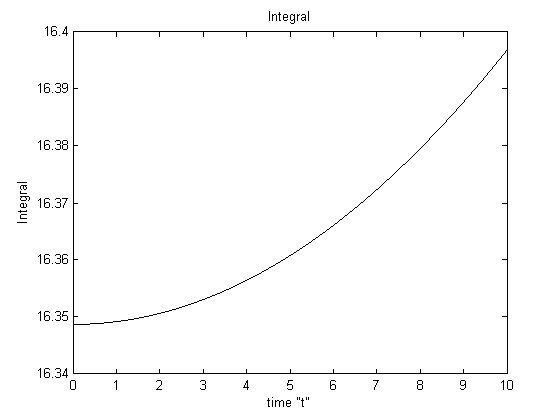
\includegraphics[width=\linewidth]{figures/Integral.png}
	\end{minipage}	
	\begin{minipage}[b]{0.4\linewidth}
		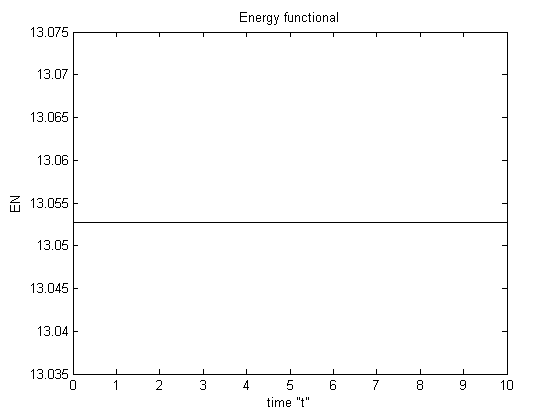
\includegraphics[width=\linewidth]{figures/Energy.png}
		
	\end{minipage}

\end{center}
The Integral  (left panel) and Energy (right panel) of the solution for Evolution of the maximum for  $\beta=1$ and $c = 0.9$.
\end{frame}

\begin{frame}
\frametitle{Results}
\framesubtitle{Wave Evolution}
\begin{center}\vspace{0.4cm}
	\begin{minipage}[b]{0.30\linewidth}
		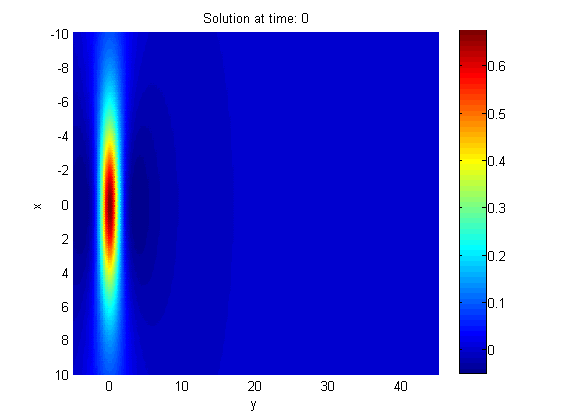
\includegraphics[width=\linewidth]{figures/Solution1_t=0.png}
	\end{minipage}	
	\begin{minipage}[b]{0.30\linewidth}
		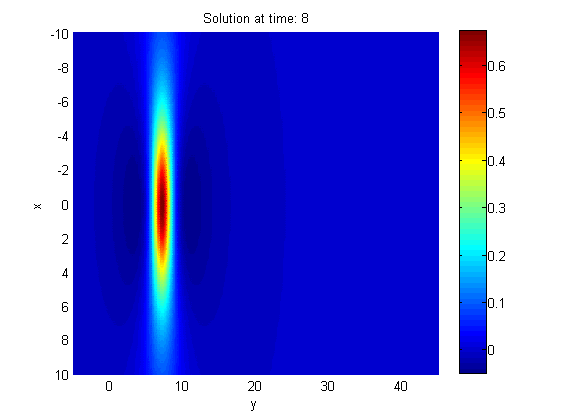
\includegraphics[width=\linewidth]{figures/Solution1_t=8.png}
	\end{minipage}	
	\begin{minipage}[b]{0.30\linewidth}
		 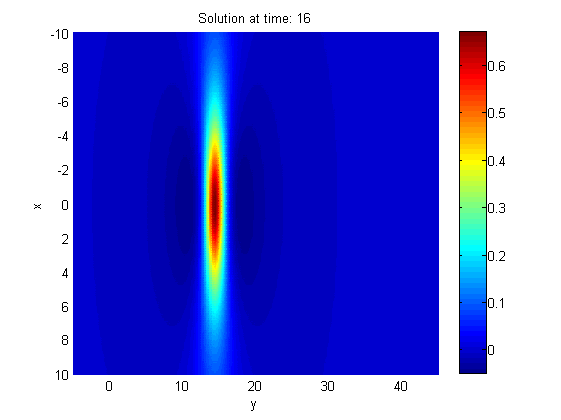
\includegraphics[width=\linewidth]{figures/Solution1_t=16.png}
	\end{minipage}
	\begin{minipage}[b]{0.30\linewidth}
		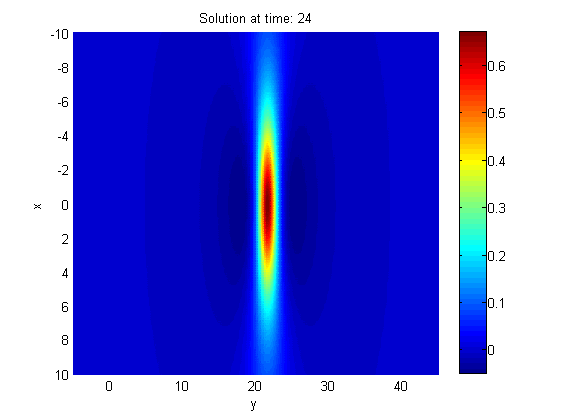
\includegraphics[width=\linewidth]{figures/Solution1_t=24.png}
	\end{minipage}	
	\begin{minipage}[b]{0.30\linewidth}
		 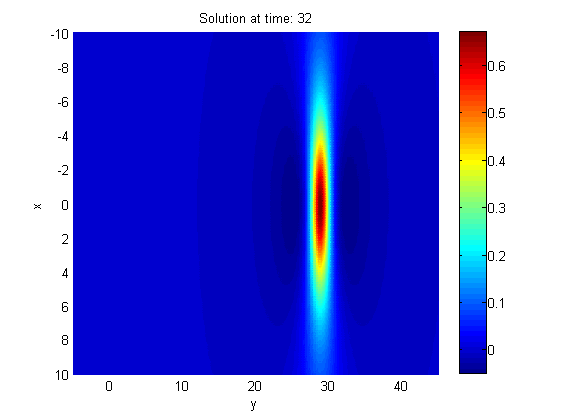
\includegraphics[width=\linewidth]{figures/Solution1_t=32.png}
	\end{minipage}
	\begin{minipage}[b]{0.30\linewidth}
		 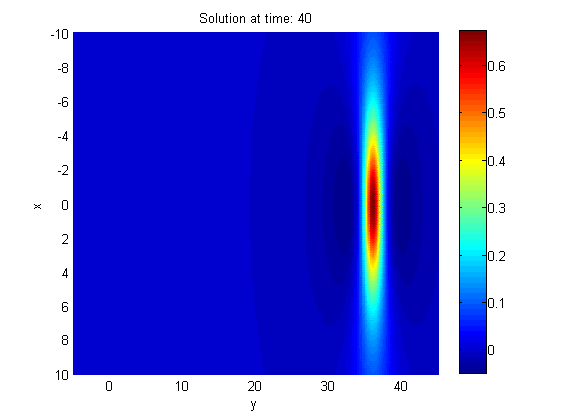
\includegraphics[width=\linewidth]{figures/Solution1_t=40.png}
	\end{minipage}
%\captionof{figure}{\color{Green} Numerical solution of single wave for $\beta=1$ and $c = 0.9$ at times $t=0,8,16,24,32,40$.}
%	\caption{Numerical solution of single wave for $\beta=1$ and $c = 0.9$ at times $t=0,8,16,24,32,40$.}
%	\label{fig:oneWaveA}
%\end{figure}
\end{center}
Numerical solution of single wave for $\beta=1$ and $c = 0.9$ at times $t=0,8,16,24,32,40$.
\end{frame}





\end{document}

